\documentclass[11pt,a4paper]{article}

\usepackage[T1]{fontenc}
\usepackage[utf8]{inputenc}
\usepackage{lmodern}
\usepackage[margin=2.5cm]{geometry}
\usepackage{amsmath}
\usepackage{graphicx}
\usepackage{booktabs}
\usepackage{tabularx}
\usepackage{longtable}
\usepackage{multirow}
\usepackage{siunitx}
\usepackage{xcolor}
\usepackage{caption}
\usepackage{subcaption}
\usepackage{enumitem}
\usepackage{listings}
\usepackage[numbers,sort&compress]{natbib}
\usepackage[colorlinks=true,linkcolor=blue!50!black,citecolor=blue!50!black,urlcolor=blue!50!black]{hyperref}
\usepackage[capitalise,noabbrev]{cleveref}

\sisetup{detect-all, separate-uncertainty=true, range-phrase=--, range-units=single}
\DeclareSIUnit\electron{e^{-}}
\DeclareSIUnit\adu{ADU}
\DeclareSIUnit\pixel{pix}

\captionsetup{font=small,labelfont=bf}
\setlist{nosep,leftmargin=*}
\lstset{basicstyle=\ttfamily\small,columns=fullflexible,keepspaces=true,
        frame=single,rulecolor=\color{black!25},xleftmargin=0.5em,xrightmargin=0.5em}

\newcommand{\pypeit}{\textsc{PypeIt}}
\newcommand{\code}[1]{\texttt{#1}}

% Generated by scripts/make_tables.py -- do not edit
\newcommand{\reportdate}{September 2026}
\newcommand{\nOHlines}{300}
\newcommand{\nBiasEpochs}{5}
\newcommand{\nFramesSurvey}{293}
\newcommand{\ronAmpOne}{\num{6.44 \pm 0.11}}
\newcommand{\ronAmpTwo}{\num{6.85 \pm 0.10}}
\newcommand{\ronExcessRange}{35--38}
\newcommand{\gainAmpOne}{\num{1.65 \pm 0.01}}
\newcommand{\gainAmpTwo}{\num{1.44 \pm 0.01}}
\newcommand{\nPtcRejected}{4}
\newcommand{\gainAgreement}{2}
\newcommand{\ptcBest}{VPH-All 1.0\_center flats of e180403\_04 (10s)}
\newcommand{\biasLevelSpread}{400}
\newcommand{\biasLevelNightly}{3}
\newcommand{\biasResidMax}{2}
\newcommand{\edgeExtraOne}{12--17}
\newcommand{\edgeExtraTwo}{2028--2033}
\newcommand{\darkRate}{7.2--25.8}
\newcommand{\darkExptimes}{120--900}
\newcommand{\satLevel}{96336}
\newcommand{\nSegLongslit}{4}
\newcommand{\segLengthArcsec}{60}
\newcommand{\bridgePix}{6}
\newcommand{\nSlitsBlueMos}{13}
\newcommand{\nSlitsRedMos}{7}
\newcommand{\seamRawRange}{0.8--2.4}
\newcommand{\seamNormRange}{0.01--0.08}
\newcommand{\pixelflatRMS}{0.7}
\newcommand{\rmsBlue}{0.036}
\newcommand{\rmsRed}{0.142}
\newcommand{\rmsAll}{0.220}
\newcommand{\chiFaintRedLS}{0.95}
\newcommand{\chiBrightRedLS}{1.00}
\newcommand{\chiFaintBlueMOS}{0.96}
\newcommand{\chiBrightBlueMOS}{1.10}
\newcommand{\chiFaintRedMOS}{1.03}
\newcommand{\chiBrightRedMOS}{1.18}
\newcommand{\flexRange}{-2.5 to +0.1}
\newcommand{\flexMaxAbs}{2.5}
\newcommand{\seamWaveJump}{0.009}
\newcommand{\seamWaveJumpRowMax}{0.10}
\newcommand{\sigmaChiPublished}{0.98}
\newcommand{\sigmaChiEnoise}{1.20}
\newcommand{\sigmaChiRange}{0.95--1.05}
\newcommand{\skyRedEndN}{319}
\newcommand{\skyRedEndMedian}{+0.22}
\newcommand{\skyRedEndStd}{0.80}
\newcommand{\skyOffsetMax}{0.57}
\newcommand{\nBoxesBlue}{5}
\newcommand{\nBoxesRed}{4}
\newcommand{\nSciSlitsBlue}{8}
\newcommand{\nSciSlitsRed}{3}
\newcommand{\nFramesTyped}{237}
\newcommand{\pypeitVersion}{2.0.1.dev1241+gf3a1f1d27.d20260922}


\title{Reduction of Magellan/LDSS3-C spectroscopy with \pypeit:\\
       pipeline description and commissioning results}
\author{Joaqu\'in Hern\'andez}
\date{\reportdate}

\begin{document}
\maketitle

\begin{abstract}
\noindent
We describe the support for the Low Dispersion Survey Spectrograph 3 (LDSS3-C)
on the Magellan Clay telescope that we have implemented in the open-source
spectroscopic pipeline \pypeit{}, and we report its performance on archival
Las Campanas Observatory commissioning data and on science data taken between
2018 and 2025. The three volume-phase holographic grisms (VPH-Blue, VPH-Red
and VPH-All) are supported in longslit and multi-slit mode. The pipeline
assembles the two amplifier files that LDSS3-C writes for each exposure,
classifies frames from the header, traces slits, builds flat fields,
calibrates the wavelength scale against archived arc-lamp templates, and
performs two-dimensional sky subtraction and optimal extraction. From bias
frames at \nBiasEpochs{} epochs we measure a read noise of
\ronAmpOne{} and \ronAmpTwo{}~\si{\electron} for the two amplifiers in the
Fast readout mode, consistent with the published values and
\ronExcessRange\,\% larger than the values recorded in the
\code{ENOISE} header keyword. Photon-transfer gains of \gainAmpOne{} and
\gainAmpTwo{}~\si{\electron\per\adu} agree with the \code{EGAIN} keyword.
Arc-lamp wavelength solutions of the \SI{1}{arcsec} slits reach median RMS
residuals of 0.04, 0.15 and 0.23~\AA{} for VPH-Blue, VPH-Red and VPH-All
(0.06--0.12 pixels), and sky emission lines in the calibrated science frames lie
within \skyOffsetMax~\AA{} of their laboratory wavelengths. All science slits of
the two multi-slit masks are calibrated; the slitmask alignment holes, which the
pipeline traces as slits, are not. We close with recommendations for observers
and for the observatory.
\end{abstract}

\tableofcontents
\clearpage

%======================================================================
\section{Introduction}
\label{sec:intro}

LDSS3-C is the facility imaging spectrograph of the \SI{6.5}{\metre} Magellan
Clay telescope at Las Campanas Observatory \citep{LDSS3manual}. It combines an
\SI{8.3}{arcmin} diameter field of view with laser-cut slitmasks, three VPH
grisms and a single $2048\times4096$ CCD, and it is widely used
for low-resolution optical spectroscopy of faint targets.

\pypeit{} \citep{pypeit:joss_pub,pypeit:zenodo} is a community-developed Python
pipeline that reduces data from more than 40 slit and echelle spectrographs with
a common set of algorithms: automatic slit tracing, two-dimensional
b-spline sky subtraction \citep{Kelson2003}, optimal extraction
\citep{Horne1986}, and wavelength calibration against archived templates. Adding
an instrument amounts to describing its detector, header conventions and default
parameters in a spectrograph class; the rest of the pipeline is shared and
maintained upstream.

This report documents the LDSS3-C implementation, currently hosted on the
\code{ldss3\_multigrating} branch of a fork of \pypeit{} \citep{ldss3_fork}, and
evaluates it on data of every grism. \Cref{sec:data} presents the instrument and
the data sets. \Cref{sec:procedure} describes each stage of the reduction and
the instrument-specific choices behind it. \Cref{sec:detector} reports the
detector characterisation, \cref{sec:wavecal} the wavelength-calibration
performance and \cref{sec:results} example reductions. \Cref{sec:recommend}
collects recommendations for observers and for the observatory, and
\cref{sec:issues} lists the known limitations. The scripts that produce every
number, table and figure in this report are distributed with it
\citep{ldss3_qa}.

%======================================================================
\section{Instrument and data}
\label{sec:data}

\subsection{Detector format}

The LDSS3-C CCD is read through two amplifiers, each covering half of the
detector in the spatial direction. The data system writes each amplifier to its
own FITS file, with a common exposure stem and the suffixes \code{c1} and
\code{c2} (e.g.\ \code{ccd1940c1.fits} and \code{ccd1940c2.fits}). Each file
holds $1024$ data columns and $128$ overscan columns by $4096$ rows (plus
overscan rows), with the dispersion along the long axis. After overscan
subtraction and trimming, the assembled frame is $4096\times2048$ pixels in the
\pypeit{} convention (spectral $\times$ spatial), with amplifier~1 covering spatial
pixels 0--1023 and amplifier~2 pixels 1024--2047
(\cref{fig:layout}). We refer to the boundary between the two halves as the
\emph{seam}. The plate scale is \SI{0.189}{arcsec\per\pixel}.

\begin{figure}[t]
  \centering
  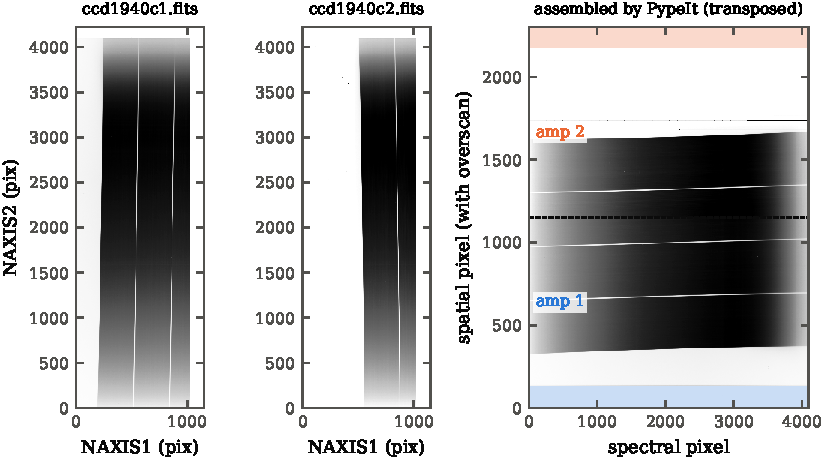
\includegraphics[width=\textwidth]{figures/detector_layout}
  \caption{A VPH-Red longslit flat (exposure 1940, 2019 February). Left: the two
    raw amplifier files as written by the instrument. Right: the frame assembled
    by \pypeit{}, before trimming, with the spectral axis horizontal. Shaded
    bands mark the overscan regions of amplifiers 1 (blue) and 2 (orange); the
    dashed line marks the seam between the two data sections.}
  \label{fig:layout}
\end{figure}

\subsection{Grisms}

\Cref{tab:grisms} summarises the three grisms as calibrated in this work. The
wavelength coverage and dispersion are measured from the arc-lamp solutions of
\cref{sec:wavecal} for a slit at the centre of the field; in multi-slit mode the
coverage shifts with the slit position along the dispersion direction.

\begin{table}[htb]
  \centering\small
  \caption{The LDSS3-C grisms as calibrated here, for the central segment of the
    \SI{1.0}{arcsec} longslit: wavelength range of the solution and range covered
    by identified arc lines, dispersion and central wavelength, arc-line FWHM and
    resolving power, and the order-blocking filter used in the data of this
    report.}
  \label{tab:grisms}
  \begin{tabular}{lccccccl}
    \toprule
    Grism & Range (\AA) & Lines (\AA) & \AA/pix & $\lambda_{\rm c}$ (\AA) & FWHM (\AA) & $R$ & Filter \\
    \midrule
    VPH-Blue & 3734--6497 & 3890--6418 & 0.690 & 5049 & 3.1 & 1611 & none \\
    VPH-Red & 5853--10588 & 5854--9787 & 1.176 & 8149 & 5.4 & 1497 & OG590 \\
    VPH-All & 2694--10620 & 3890--10473 & 2.029 & 6411 & 8.8 & 730 & none \\
    \bottomrule
  \end{tabular}
\end{table}


\subsection{Data sets}

We use five data sets (\cref{tab:datasets}). The three longslit sets come from
the Las Campanas commissioning archive and include arcs and flats for each grism,
and spectrophotometric standards for VPH-Red and VPH-All. The two multi-slit sets are science
observations: the VPH-Blue mask ATM3a2\_1 (2022 November) and the VPH-Red mask
CDFS01 (2025 December). All data were taken in the Fast readout mode with
$1\times1$ binning. Bias and dark frames from all epochs are used only for the
detector measurements of \cref{sec:detector}; they are not used in the
reductions (\cref{sec:basic}).

\begin{table}[t]
  \centering\small
  \caption{Data sets reduced for this report: number of arc, flat and
    science/standard exposures used.}
  \label{tab:datasets}
  \begin{tabular}{llllrrrl}
    \toprule
    Grism & Slit/mask & Filter & Date (UT) & Arcs & Flats & Sci. & Targets \\
    \midrule
    VPH-Blue & 1.0\_center & Open & 2019-02-19 -- 02-22 & 2 & 6 & 0 & -- \\
    VPH-Red & 1.0\_center & OG590 & 2019-02-20 & 3 & 5 & 4 & GD71 \\
    VPH-All & 1.0\_center & Open & 2018-04-03 -- 04-04 & 3 & 5 & 4 & EG274, Hiltner600 \\
    VPH-Blue & ATM3a2\_1 & Open & 2022-11-15 -- 11-16 & 2 & 7 & 4 & ATM3a2\_1 \\
    VPH-Red & CDFS01 & OG-590 & 2025-12-22 -- 12-23 & 3 & 10 & 3 & CDFS01 \\
    \bottomrule
  \end{tabular}
\end{table}


%======================================================================
\section{Reduction procedure}
\label{sec:procedure}

The reduction follows the standard \pypeit{} multi-slit path
\citep{pypeit:joss_pub}. A reduction is set up with \code{pypeit\_setup},
which reads the headers, classifies the frames and groups them into
configurations, and run with \code{run\_pypeit}. We describe each stage below,
emphasising the choices made for LDSS3-C. The complete set of default
parameters is listed in \cref{app:params}.

\subsection{Frame assembly and basic image processing}
\label{sec:basic}

During setup, \pypeit{} ingests only one file per exposure (the \code{c1}
file). When a frame is read, the companion amplifier file is located from the
file name and the two halves are joined in memory; no pre-merged files are
needed. The gain and read noise are assigned per amplifier: the gain is read
from the \code{EGAIN} keyword, and the read noise is taken from the published
value for the readout mode given by the \code{SPEED} keyword, not from the
\code{ENOISE} keyword, which we find to be incorrect (\cref{sec:ron}).

For each amplifier the overscan is subtracted row by row and the image is
trimmed to the data section. Bias frames are not subtracted by default: the
bias residuals left after overscan subtraction are below
\SI{\biasResidMax}{\adu} (\cref{fig:bpm}), and small compared with the read noise,
and subtracting a combined bias would add noise for little gain. Dark frames are likewise not
subtracted; the dark current (\cref{sec:dark}) is small and is accounted for in
the noise model. Cosmic rays are identified in science frames with the
\pypeit{} L.A.Cosmic implementation (\code{sigclip}~=~5,
\code{objlim}~=~2).

Saturation is set by the 16-bit analogue-to-digital converter, not by the full
well. The CCD full well is \SI{\sim205000}{\electron} and the response stays
linear to within \SI{1}{\percent} up to \SI{\sim175000}{\electron}, but 65535
ADU corresponds to only \SI{108133}{\electron} (amplifier~1) and
\SI{96336}{\electron} (amplifier~2). The saturation threshold is therefore set
to $65535\times\min(g_1,g_2) = \SI{\satLevel}{\electron}$, with a
non-linearity fraction of 0.99, so that saturated pixels are flagged on both
amplifiers.

\subsection{Frame classification}
\label{sec:typing}

The \code{EXPTYPE} keyword does not distinguish reliably between calibration
types: arcs and flats are written both with \code{EXPTYPE = 'Flat'} and with
\code{EXPTYPE = 'Object'}, depending on how the exposure was started, and
bias frames carry whatever grism was in the beam. Frames are therefore
classified by combining \code{EXPTYPE} with keywords in the \code{OBJECT}
card (\cref{tab:typing}). Short keywords must appear as separate words
(delimited by spaces, underscores or hyphens), so that, e.g., a target named
``Arcturus'' is not taken for an arc; \code{flat}, \code{quartz} and
\code{dome} are matched anywhere in the name, which catches \code{flatQh}.
Frames taken without a grism (acquisition, through-slit and direct images) are
discarded. Science frames and standards are separated by exposure time, at
\SI{100}{\second} by default.

\begin{table}[t]
  \centering\small
  \caption{Frame classification from the \code{OBJECT} card.}
  \label{tab:typing}
  \begin{tabular}{lll}
    \toprule
    \code{OBJECT} contains & Frame type & Examples from the archive \\
    \midrule
    \code{arc}, \code{arcs}, \code{henear}, \code{hene}, \code{lamp}, \code{comp}
      & arc, tilt & ``arc ATM3a2\_1'', ``GD71 VPH-RED OG590 Arc'' \\
    \code{flat}, \code{quartz}, \code{dome}, \code{qh}, \code{ff}
      & pixel flat, illumination flat, trace & ``EG274 - Qh'', ``LTT3218 flatQh'' \\
    \code{zero}, \code{bias} & bias & ``Zero'', ``Bias'' \\
    \code{dark} & dark & ``Dark'' \\
    \code{align}, \code{thr}, \code{field}, \code{focus}, \code{acq} & ignored & ``align MASK'' \\
    anything else & science or standard & ``science ATM3a2\_1'', ``EG274 - spec'' \\
    \bottomrule
  \end{tabular}
\end{table}

We inspected the classification of all frames in the configurations used here.
Two frames were misclassified: an arc named ``Hiltner600 - NeHeAr'', typed as a
standard because \code{nehear} is not among the keywords, and a \SI{1}{\second}
test exposure named ``Tests'', typed as a standard. The first was retyped and
the second removed by hand in the input file, which is the supported way of overriding the automatic
classification (\cref{sec:recommend}).

A configuration is defined by the grism, the slitmask (\code{APERTURE}), the
binning and the order-blocking filter. The filter is included because it changes
the spectral shape of the flat field; frames taken with different filters are
never calibrated together automatically (see \cref{sec:flat}).

\subsection{Bad-pixel mask}
\label{sec:bpm}

The default bad-pixel mask flags twelve column ranges (\cref{tab:bpm}),
including the outer edge columns of each amplifier. They were identified from
the column profile of combined biases and confirmed at \nBiasEpochs{} epochs
between 2018 and 2025 (\cref{fig:bpm}). Flagging columns that deviate from
the local median by more than 8 times the column-to-column scatter, every masked
range is detected in at least four of the five epochs. The only other columns
detected that often are \edgeExtraOne{} and \edgeExtraTwo, adjacent to the masked
outer edges of the detector; they lie in the edge roll-off and are not inside any
slit in the data analysed here. Apart from these columns, the overscan-subtracted
bias is flat to within \SI{\biasResidMax}{\adu}, with a smooth gradient of about
\SI{1.5}{\adu} towards the seam.

\begin{table}[t]
  \centering\small
  \caption{Columns masked by default, in pixels of the trimmed, unbinned frame
    (spatial axis; amplifier~1 is 0--1023).}
  \label{tab:bpm}
  \begin{tabular}{lrclrc}
    \toprule
    Columns & $N$ & Amp. & Columns & $N$ & Amp. \\
    \midrule
    0--11 & 12 & 1 & 1602--1606 & 5 & 2 \\
    443 & 1 & 1 & 1635--1640 & 6 & 2 \\
    608 & 1 & 1 & 1688--1690 & 3 & 2 \\
    1413 & 1 & 2 & 1695 & 1 & 2 \\
    1492--1494 & 3 & 2 & 1999--2000 & 2 & 2 \\
    1549--1551 & 3 & 2 & 2034--2047 & 14 & 2 \\
    \bottomrule
  \end{tabular}
\end{table}


\begin{figure}[t]
  \centering
  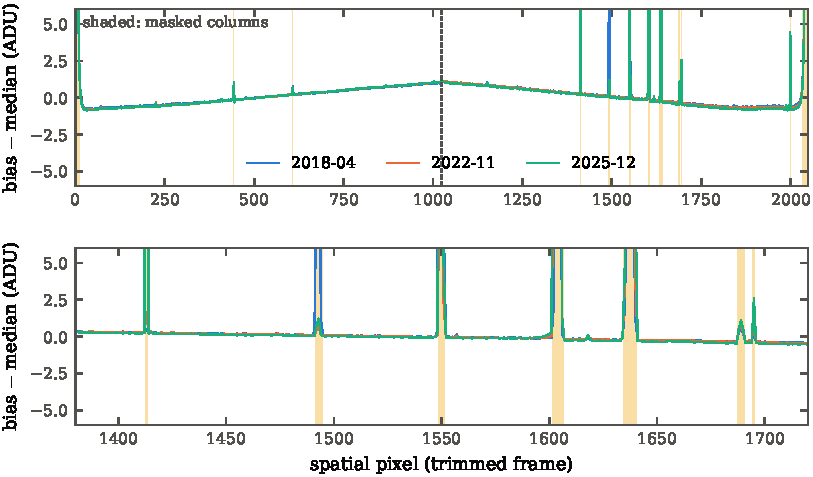
\includegraphics[width=\textwidth]{figures/bias_bpm}
  \caption{Column profile of combined, overscan-subtracted bias frames at three
    epochs, relative to the median of amplifier~1. Shaded columns are those
    masked by default. The lower panel is an enlargement of the region with most
    bad columns. The dashed line marks the seam.}
  \label{fig:bpm}
\end{figure}

\subsection{Slit tracing}
\label{sec:slits}

Slit edges are found in the combined trace flat from the spatial gradient of
the illumination and followed along the dispersion direction. For LDSS3-C the
edge-detection threshold is raised to \code{edge\_thresh}~=~20: at lower
thresholds, bad columns and the detector edges produce spurious narrow slits.
Slits shorter than \SI{2}{arcsec} (\code{minimum\_slit\_length}) are rejected;
the narrowest real slitlets we have encountered are \SI{\sim5}{arcsec} long. In
multi-slit mode, missing edges are predicted from a principal-component model of
the other slits; for the longslit masks (\code{APERTURE} containing
\code{center} or \code{long}) the prediction uses the nearest traced slit
instead.

The LDSS3-C longslits are not continuous: the slit is cut in segments separated
by narrow bridges that hold the mask together. \pypeit{} traces each segment as
a separate slit (\cref{fig:slits}, left). For the \SI{1.0}{arcsec}
\code{center} slit we find \nSegLongslit{} segments of
\SI{\segLengthArcsec}{arcsec} each, separated by bridges of
\SI{\sim\bridgePix}{\pixel}. This has no practical consequence for the
reduction, but an object that falls on a bridge is lost, and each segment
receives its own wavelength solution.

\Cref{fig:slits} also shows the two multi-slit masks, which we compared with
their design files. ATM3a2\_1 has 8 slits of $1\times\SI{6}{arcsec}$ and 6
alignment holes of \SI{5}{arcsec} diameter; CDFS01 has 3 slits of
$1\times\SI{12}{arcsec}$ and 9 holes. All science slits were traced
(\nSciSlitsBlue{} and \nSciSlitsRed). The alignment holes are also traced, as
short slits: \nBoxesBlue{} in ATM3a2\_1 and \nBoxesRed{} in CDFS01, where
several holes share the same spatial position. The holes are
wider than the slits in the dispersion direction, so they are over-exposed in
flats and arcs and their arc lines are broad; they cannot be calibrated and must
be ignored (\cref{sec:holes}). A slit whose edge falls on a masked bad column
cannot be traced there and may be lost; this did not occur for the two masks
studied, but should be considered in mask design (\cref{sec:recommend}).

\begin{figure}[t]
  \centering
  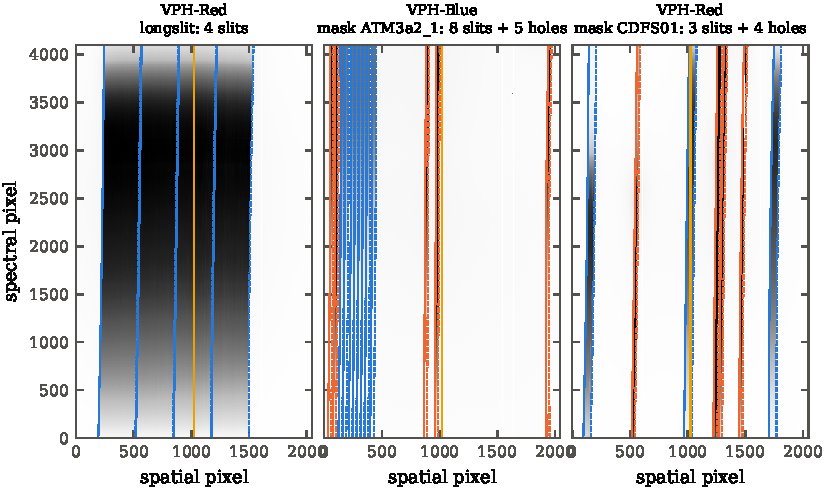
\includegraphics[width=\textwidth]{figures/slit_edges}
  \caption{Traced slit edges (solid: left edge; dashed: right edge) over the
    combined trace flat, for the VPH-Red longslit and the two multi-slit masks.
    Slits flagged by the pipeline are shown in orange. The yellow line marks the
    seam.}
  \label{fig:slits}
\end{figure}

\subsection{Flat fielding}
\label{sec:flat}

The flat-field frames (internal quartz lamp; \code{Qh} in the LDSS3
nomenclature) are combined and decomposed, slit by slit, into a spectral
response, a spatial illumination profile and a pixel-to-pixel sensitivity
map (\cref{fig:flat}). The pixel flat corrects for pixel-scale
sensitivity variations with an RMS of \pixelflatRMS\,\% in the VPH-Red
longslit data.

Because the two amplifiers have slightly different gains, a flat shows a
step at the seam. Measured inside the longslit segment that crosses the seam, it
is \seamRawRange\,\% in the combined flats and \seamNormRange\,\% after
normalisation, confirming that the two halves are joined and scaled
consistently. None of the multi-slit slits spans enough of the seam for the
measurement.

The last step of the illumination model is a fine correction of the spatial
profile of each slit, fitted in bins of wavelength. It is the step most sensitive
to the quality of the flat, and its QA plots
(\code{QA/PNGs/Spatillum\_FineCorr\_*}) should be inspected. In the data analysed
here, inspected slit by slit, the correction amounts to
\SIrange{1}{2}{\percent} across the slit in the longslit segments and in the
science slits of ATM3a2\_1, and follows the data smoothly. In the science slits of
CDFS01, whose flats were taken without the blocking filter (see below), it
reaches \SIrange{3}{4}{\percent} and is fitted to visibly noisier profiles. It
fails in two recognisable ways, both in alignment holes. Where the flat is
saturated, only the unsaturated part of the aperture enters the fit and the
profile is extrapolated over the rest; this occurs in the holes of CDFS01,
whose flats reach the ADC ceiling. In ATM3a2\_1, one wavelength bin of one hole
shows a spurious gradient of \SI{\sim3}{\percent}.

The VPH-Red flats of CDFS01 were taken without the OG-590 order-blocking filter
used for the arcs and science frames. Such frames form a separate configuration
and are not associated automatically; for this report we combined them by hand.
This is adequate for the pixel-to-pixel correction and for slit tracing, but the
spectral shape of an unfiltered flat differs from that of the science data below
\SI{\sim6000}{\angstrom}, and the extra light is what saturates the alignment holes.
Flats should be taken with the same filter as the science
(\cref{sec:recommend}).

\begin{figure}[t]
  \centering
  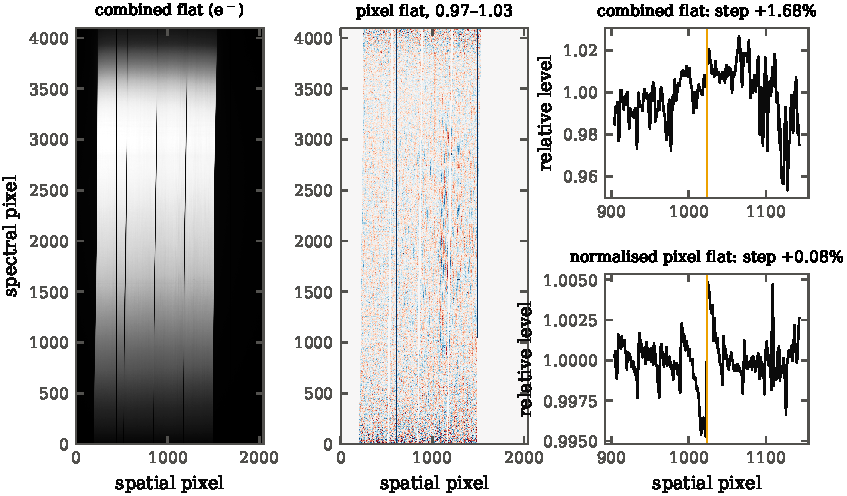
\includegraphics[width=\textwidth]{figures/flat}
  \caption{Flat field for the VPH-Red longslit. Left: combined flat (in
    electrons). Centre: normalised pixel-to-pixel flat. Right: median spatial
    profile around the seam before (top) and after (bottom) normalisation; the
    quoted step is measured by extrapolating a linear fit from each side to the
    seam.}
  \label{fig:flat}
\end{figure}

\subsection{Wavelength calibration}
\label{sec:wavecal_method}

Arc spectra are extracted along the centre of each slit, and the lines are
detected above a threshold of \code{sigdetect}~=~6 with an expected FWHM of
\SI{6}{\pixel}. The wavelength solution is found with the \code{full\_template}
method: the arc spectrum of each slit is cross-correlated with an archived
template for the same grism (\cref{fig:templates}), allowing for a shift and a
stretch, and the template's identified lines are transferred to the observed
spectrum within a tolerance of \SI{2.5}{\pixel}. A Legendre polynomial of order
\code{n\_final}~=~5 is then fitted to the pixel positions of the identified
lines, with iterative rejection of outliers; solutions with an RMS larger than
half the line FWHM are rejected. The line lists are those distributed with
\pypeit{} for the HeI, NeI and ArI lamps, in vacuum wavelengths \citep{NIST_ASD}.

The templates are HeNeAr spectra of the \SI{1}{arcsec} longslit, one per
grism, whose wavelength scales were checked against the reference arc
identifications distributed by Las Campanas Observatory for each grism. They
cover the full detector. Because the template is matched to each slit, the
same template serves slits at any position on a multi-slit mask.

The wavelength solution is extended to two dimensions by tracing the arc lines
along each slit and fitting the line tilts with a two-dimensional polynomial of
order 6 in both directions.

\subsection{Sky subtraction and extraction}
\label{sec:skysub}

The sky is modelled in two dimensions, slit by slit, with a b-spline in the
wavelength--spatial plane \citep{Kelson2003} with a break-point spacing of
0.8 pixels. Objects are found in the sky-subtracted image and extracted with both
a boxcar and an optimal extraction \citep{Horne1986}; in the second pass the sky
is re-fitted jointly with the object profiles. For standard stars the global sky
subtraction is skipped. On multi-slit data we recommend excluding the outer
parts of each slitlet from the object search to avoid spurious detections at the
edges (\code{find\_trim\_edge}; \cref{app:quickstart}).

\subsection{Flexure correction}
\label{sec:flexure}

Arcs are usually taken at a different telescope position from the science
frames, so a residual shift in the spectral direction is expected. It is measured
by cross-correlating the extracted sky spectrum of each object with an archived
sky spectrum and applied to the wavelength scale (\code{spec\_method}~=~
\code{boxcar}). For the science slits in this study the measured shifts range
from \flexRange{}~pixels. The largest, about \SI{-2.4}{\pixel}, is common to all
slits of CDFS01, for arcs taken during the night close to the science
exposures; it is confirmed independently by the sky lines (\cref{sec:zeropoint}).
Standards are not corrected. Flexure should be checked in the QA plots
(\code{QA/PNGs/*spec\_flex\_corr*}).

\subsection{Flux calibration}
\label{sec:flux}

Sensitivity functions are computed with \code{pypeit\_sensfunc} using the
\code{IR} algorithm, which fits the instrument response jointly with a
telluric model, with a polynomial of order 7. The flux calibration
has not been validated and is not assessed in this report.

%======================================================================
\section{Detector characterisation}
\label{sec:detector}

\subsection{Header keywords}

All \nFramesSurvey{} exposures surveyed here, from 2018 April to 2025 December,
carry the same detector keywords: \code{SPEED = 'Fast'},
\code{EGAIN}~=~1.65 and 1.47~\si{\electron\per\adu}, and
\code{ENOISE}~=~4.67 and 5.06~\si{\electron} for amplifiers 1 and 2. The
\code{ENOISE} values are close to the published Slow-mode values, not to the Fast-mode ones. The published
read noise is \SIlist{4.4;5.3}{\electron} (Slow),
\SIlist{7.0;7.2}{\electron} (Fast) and \SI{\sim10}{\electron} (Turbo) for the
two amplifiers.

\subsection{Read noise}
\label{sec:ron}

The read noise was measured at \nBiasEpochs{} epochs from the differences of
consecutive bias frames, $\sigma_{\rm RN}=\sigma(B_i-B_{i+1})/\sqrt2$, in the
central region of each amplifier after overscan subtraction, with iterative
$4\sigma$ clipping. It was also measured independently from the scatter in the
overscan. The results are listed in \cref{tab:ron} and shown in
\cref{fig:ron}. The mean over epochs is \ronAmpOne{} and
\ronAmpTwo~\si{\electron}, consistent with the published Fast values and
\ronExcessRange\,\% larger than the \code{ENOISE} keyword.

\begin{table}[t]
  \centering\small
  \caption{Read noise (\si{\electron}) per epoch, from bias-pair differences
    (mean $\pm$ standard deviation over pairs) and from the overscan scatter, for
    the gains in the \code{EGAIN} keyword. The published Fast-mode values are 7.0
    and 7.2~\si{\electron}; the \code{ENOISE} keyword gives 4.67 and
    5.06~\si{\electron}.}
  \label{tab:ron}
  \begin{tabular}{lrcccc}
    \toprule
    & & \multicolumn{2}{c}{Amplifier 1} & \multicolumn{2}{c}{Amplifier 2} \\
    \cmidrule(lr){3-4}\cmidrule(lr){5-6}
    Epoch & $N_{\rm bias}$ & pairs & overscan & pairs & overscan \\
    \midrule
    2018 Apr & 5 & \num{6.43 \pm 0.10} & 6.21 & \num{6.82 \pm 0.12} & 6.56 \\
    2019 Dec & 5 & \num{6.74 \pm 0.26} & 6.62 & \num{7.13 \pm 0.26} & 6.94 \\
    2020 Nov & 5 & \num{6.61 \pm 0.84} & 6.72 & \num{7.03 \pm 0.81} & 7.11 \\
    2022 Nov & 10 & \num{6.24 \pm 0.39} & 6.09 & \num{6.67 \pm 0.42} & 6.46 \\
    2025 Dec & 13 & \num{6.17 \pm 0.26} & 6.17 & \num{6.62 \pm 0.28} & 6.54 \\
    \midrule
    Mean & & \num{6.44 \pm 0.11} & & \num{6.85 \pm 0.10} & \\
    \bottomrule
  \end{tabular}
\end{table}


\begin{figure}[t]
  \centering
  \begin{minipage}[t]{0.49\textwidth}
    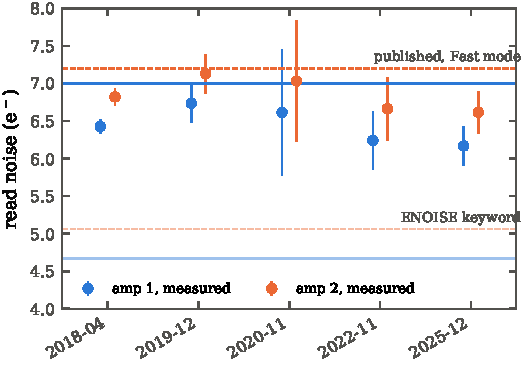
\includegraphics[width=\textwidth]{figures/readnoise}
    \caption{Read noise measured from bias pairs at each epoch. Horizontal lines
      are the published Fast-mode values (upper) and the \code{ENOISE} keyword
      values (lower) for amplifier~1 (solid) and 2 (dashed).}
    \label{fig:ron}
  \end{minipage}\hfill
  \begin{minipage}[t]{0.49\textwidth}
    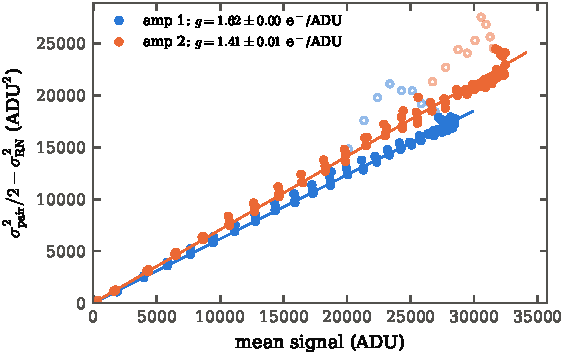
\includegraphics[width=\textwidth]{figures/ptc}
    \caption{Photon-transfer curve for \ptcBest. Filled points are used in the
      fit; the lines have slope $1/g$.}
    \label{fig:ptc}
  \end{minipage}
\end{figure}

The read noise enters the variance of every pixel, so the choice matters most
where the sky is faint, in the blue and between the sky lines. We tested it with
the distribution of $\chi = (d - s - o)\sqrt{w}$ over the sky-dominated pixels of
the science exposures (excluding the alignment holes), where $d$, $s$ and $o$ are
the data, the sky model and the object model and $w$ is the inverse variance.
With the published read noise the distribution has a standard deviation of
\sigmaChiPublished{} (\sigmaChiRange{} for individual exposures). Replacing the
read noise with the \code{ENOISE} values gives \sigmaChiEnoise{}: the
uncertainties would be underestimated by \SI{20}{\percent} (\cref{fig:noise}).
Standard stars are excluded from this test because they are reduced without a
global sky model. The pipeline therefore
takes the read noise from the readout mode and falls back on \code{ENOISE},
with a warning, only for an unrecognised mode.

\begin{figure}[t]
  \centering
  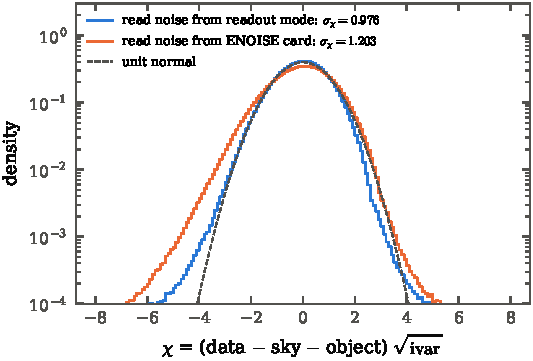
\includegraphics[width=0.62\textwidth]{figures/noise_model}
  \caption{Distribution of the normalised residuals $\chi$ over the good pixels
    of the science frames in \cref{tab:datasets}, for the variance computed with
    the published read noise (as used by the pipeline) and with the
    \code{ENOISE} header values. The dashed line is a unit normal.}
  \label{fig:noise}
\end{figure}

\subsection{Gain}
\label{sec:gain}

The gain was measured with the photon-transfer method \citep{Janesick2007} from
pairs of flats with identical set-up and exposure time. For each pair, the
second frame was scaled to the median level of the first, the pixels were binned
by mean signal, and the variance of the pair difference was compared with the
signal in each bin, after subtracting the read-noise term. Only pixels where the
illumination is locally smooth (gradient below \SI{0.5}{\percent} per pixel)
were used, so that small shifts of the slit image between the two exposures do
not add variance. \Cref{fig:ptc} shows an example and \cref{tab:gain} lists the
results. Eight of the twelve sets give consistent gains. Of the other
\nPtcRejected, three (all from the 2025 December run) depart from \code{EGAIN}
by more than \SI{10}{\percent} and have curved transfer curves, which indicates
that the illumination changed between the two exposures of a pair in a way that a
single scale factor does not remove; the fourth has too few usable points on one
amplifier. The mean of the consistent sets is \gainAmpOne{} and \gainAmpTwo~\si{\electron\per\adu},
in agreement with \code{EGAIN} (1.65 and 1.47) to within \gainAgreement\,\%. The
pipeline uses \code{EGAIN}.

\begin{table}[t]
  \centering\small
  \caption{Gain (\si{\electron\per\adu}) from photon-transfer curves of flat pairs.
    Uncertainties are bootstrap estimates for each set. Sets marked $\dagger$
    depart from \code{EGAIN} by more than 10\,\% on at least one amplifier,
    because the lamp or illumination changed between the exposures of a pair, and
    are excluded from the mean.}
  \label{tab:gain}
  \begin{tabular}{llllrcc}
    \toprule
    Night & Grism & Slit/mask & $t_{\rm exp}$ & Pairs & Amp.~1 & Amp.~2 \\
    \midrule
    e180403\_04 & VPH-All & 1.0\_center & 10s & 4 & \num{1.619 \pm 0.005} & \num{1.414 \pm 0.006} \\
    e190218\_19 & VPH-Blue & 1.0\_center & 70s & 3 & \num{1.632 \pm 0.006} & \num{1.437 \pm 0.004} \\
    e190219\_20 & VPH-Blue & 1.0\_center & 70s & 1 & \num{1.652 \pm 0.003} & \num{1.452 \pm 0.005} \\
    e190219\_20 & VPH-Red & 1.0\_center & 14s & 1 & \num{1.654 \pm 0.004} & \num{1.464 \pm 0.004} \\
    e190219\_20 & VPH-Red & 1.0\_center & 8s & 1 & \num{1.650 \pm 0.003} & \num{1.460 \pm 0.003} \\
    e201124\_25 & VPH-Blue & 1.0\_center & 70s & 1 & \num{1.664 \pm 0.004} & \num{1.444 \pm 0.005} \\
    nov22\_atm3a2 & VPH-Blue & ATM3a2\_1 & 70s & 3 & \num{1.594 \pm 0.005} & \num{1.393 \pm 0.014}$^\dagger$ \\
    nov22\_atm3a2 & VPH-Blue & ATM3a2\_1 & 80s & 1 & \num{1.642 \pm 0.007} & \num{1.420 \pm 0.005} \\
    ut251222\_23 & VPH-Red & 1.00\_center & 14s & 4 & \num{0.857 \pm 0.068} & \num{0.601 \pm 0.053}$^\dagger$ \\
    ut251222\_23 & VPH-Red & CDFS01 & 14s & 4 & \num{1.626 \pm 0.024} & \num{1.117 \pm 0.111}$^\dagger$ \\
    ut251222\_23 & VPH-Red & CDFS03 & 14s & 4 & \num{0.736 \pm 0.053} & \num{0.715 \pm 0.048}$^\dagger$ \\
    ut251222\_23 & VPH-Red & CDFS05 & 14s & 4 & \num{1.672 \pm 0.006} & \num{1.424 \pm 0.009} \\
    \midrule
    \multicolumn{5}{l}{Mean of accepted sets} & \num{1.65 \pm 0.01} & \num{1.44 \pm 0.01} \\
    \multicolumn{5}{l}{\code{EGAIN}} & 1.65 & 1.47 \\
    \bottomrule
  \end{tabular}
\end{table}


\subsection{Bias level and dark current}
\label{sec:dark}

The overscan level differs between epochs by up to \biasLevelSpread~ADU, and
within a night it is stable to better than \SI{\biasLevelNightly}{\adu}, which
justifies the row-by-row overscan subtraction without a bias frame. The dark
current, measured from dark exposures of \darkExptimes~s bracketed by biases
(sigma-clipped mean of the difference), is \darkRate~\si{\electron\per\pixel\per\hour},
with amplifier~2 consistently about twice amplifier~1. The pipeline adopts
\SI{25}{\electron\per\pixel\per\hour} in its noise model. For a
\SI{20}{min} exposure this amounts to \SIrange{2}{9}{\electron} per pixel, well
below the sky level in any spectroscopic exposure but not negligible compared
with the read noise, so the dark current is included in the variance but not
subtracted.

%======================================================================
\section{Wavelength-calibration performance}
\label{sec:wavecal}

\Cref{fig:templates} shows the three arc templates with the lines used in the
solution, and \cref{fig:residuals} shows the residuals of the longslit
solutions. \Cref{tab:wavecal} summarises the performance for every data set.
For the multi-slit masks, \cref{fig:mos_wavecal} shows the dispersion, number of
lines and RMS of every slit.

\begin{figure}[p]
  \centering
  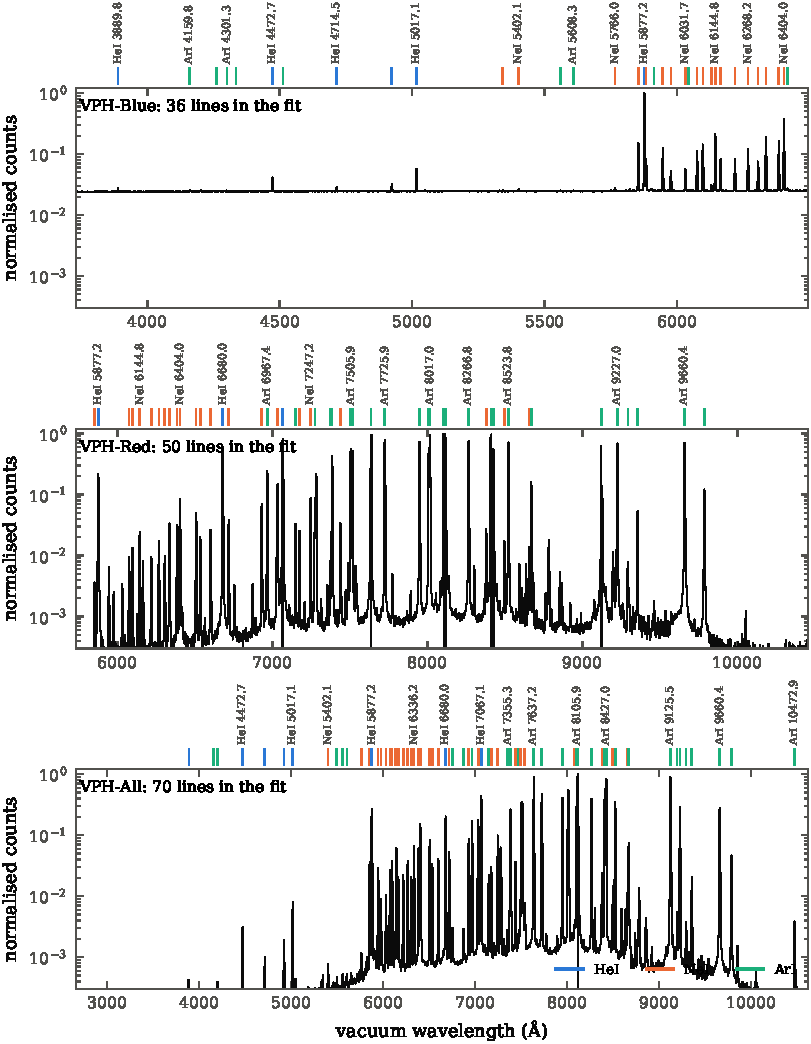
\includegraphics[width=\textwidth]{figures/arc_templates}
  \caption{Archived HeNeAr arc templates for the three grisms, with the lines used
    in the wavelength solution of the longslit data marked by element (HeI blue,
    NeI orange, ArI green). The brightest lines are labelled with their vacuum
    wavelength in \AA.}
  \label{fig:templates}
\end{figure}

\begin{figure}[t]
  \centering
  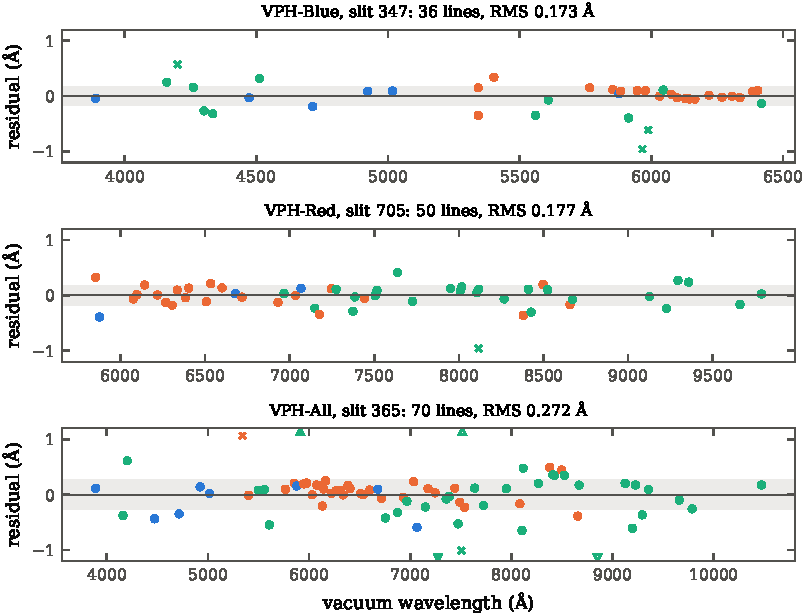
\includegraphics[width=\textwidth]{figures/wavecal_residuals}
  \caption{Residuals of the wavelength solutions for the longslit data, for the
    slit segment with the most identified lines. Filled symbols are lines used in
    the fit, crosses are rejected lines; the shaded band is $\pm$RMS.}
  \label{fig:residuals}
\end{figure}

\begin{table}[t]
  \centering\small
  \caption{Wavelength-calibration performance. For each data set and calibration
    group: slits with a valid solution out of the science slits traced (alignment
    holes excluded); and, as medians over
    those slits, the number of lines in the fit, the RMS residual in \AA, pixels
    and \si{\kilo\metre\per\second}, the FWHM of the arc lines and the resolving
    power $R=\lambda_{\rm c}/{\rm FWHM}$ at the central wavelength for the
    \SI{1}{arcsec} slit.}
  \label{tab:wavecal}
  \begin{tabular}{lcccccccc}
    \toprule
    Data set & Group & Slits & $N_{\rm lines}$ & RMS (\AA) & RMS (pix) & RMS (km/s) & FWHM (\AA) & $R$ \\
    \midrule
    VPH-Blue, 1.0'' longslit & 0 & 4/4 & 31 & 0.045 & 0.06 & 3 & 3.2 & 1576 \\
    VPH-Blue, 1.0'' longslit & 1 & 4/4 & 26 & 0.042 & 0.06 & 2 & 3.2 & 1580 \\
    VPH-Red, 1.0'' longslit & 0 & 4/4 & 46 & 0.147 & 0.12 & 5 & 5.5 & 1480 \\
    VPH-All, 1.0'' longslit & 0 & 4/4 & 66 & 0.245 & 0.12 & 11 & 8.7 & 736 \\
    VPH-All, 1.0'' longslit & 1 & 4/4 & 60 & 0.218 & 0.11 & 10 & 8.7 & 738 \\
    VPH-Blue, mask ATM3a2\_1 & 0 & 8/8 & 41 & 0.077 & 0.11 & 5 & 3.2 & 1573 \\
    VPH-Red, mask CDFS01 & 0 & 3/3 & 52 & 0.082 & 0.07 & 3 & 6.2 & 1321 \\
    \bottomrule
  \end{tabular}
\end{table}


\paragraph{VPH-Blue.} The solution is constrained by HeI, NeI and ArI lines from
\SIrange{3890}{6418}{\angstrom}, with 26--44 lines per slit and a median RMS of
0.04--0.08~\AA{} per data set (\SI{\sim0.1}{\pixel}; 0.04--0.17~\AA{} for individual
slits). The blue half of the range has few, faint
lines (\cref{fig:templates}), so the solution there relies on HeI 3889, 4472,
4714 and 5017~\AA{} and ArI 4159 and 4301~\AA; the Ne lines cluster redward of
\SI{5800}{\angstrom}. In ATM3a2\_1 the eight science slits give dispersions within
\SI{0.5}{\percent} of each other and coverage that shifts by up to
\SI{110}{\angstrom} with slit position.

\paragraph{VPH-Red.} Lines from \SIrange{5854}{9787}{\angstrom} constrain the
solution, with 36--62 lines per slit and an RMS of 0.05--0.18~\AA. The reddest
\SI{\sim800}{\angstrom} of the detector, beyond the last strong ArI line, are
extrapolated. The sky lines show that the extrapolation is adequate: the
\skyRedEndN{} sky-line measurements redward of \SI{9800}{\angstrom} give a median
offset of \skyRedEndMedian~\AA{} (scatter \skyRedEndStd~\AA). Slits placed so
that their spectra start blueward of the first arc line are also extrapolated at
the blue end; in CDFS01 the [OI] \SI{5577}{\angstrom} sky line is found
\SI{1.5}{\angstrom} too blue there, in a range the OG-590 filter blocks anyway.

\paragraph{VPH-All.} The coverage of VPH-All is limited by the arc lamps, not by
the detector: lines are identified from \SIrange{3890}{10473}{\angstrom}, and the
first \SI{\sim600}{\pixel} (below \SI{3890}{\angstrom}) are extrapolated, where
the grism has no throughput and no signal is recorded. With 60--70 lines per slit
the RMS is 0.19--0.27~\AA, or \SI{0.1}{\pixel}.

\paragraph{Continuity across the seam.} Extrapolating the wavelength image from each
side to the seam, the median discontinuity over the rows of a slit is at most
\seamWaveJump~\AA, and the largest in any single row is \seamWaveJumpRowMax~\AA{}
(\SI{0.08}{\pixel}, in the CDFS01 slit that crosses the seam), well below the
dispersion.

\subsection{Alignment holes}
\label{sec:holes}

The alignment holes of a slitmask are traced as short slits
(\cref{sec:slits}). Because they are much wider than a slit in the dispersion
direction, their arc lines are broad and flat-topped, often saturated, and the
template match fails or produces a wrong solution (\cref{fig:mos_wavecal}). Such
a solution can still have a small RMS if it matches a few lines, so the
dispersion and the line width, rather than the RMS, identify it: in both masks
every hole has an arc-line FWHM more than 1.5 times that of the slits or a
failed solution, and no science slit does. \code{ldss3\_qa.py} flags these
apertures automatically. Objects found in them are the alignment stars.

\subsection{Zero point from the sky lines}
\label{sec:zeropoint}

The arc solutions are applied to science frames taken at other times and
telescope positions, corrected for flexure (\cref{sec:flexure}). To test the
final wavelength scale independently of the arcs, we fitted Gaussian profiles to
isolated sky emission lines in the extracted sky spectrum of every science slit:
the [OI] lines at 5577, 6300 and \SI{6364}{\angstrom} and the brightest OH lines
of \code{OH\_LDSS3\_vac} with no other listed line within \SI{8}{\angstrom}
(after removing the heliocentric correction applied by the pipeline). Fits with
widths inconsistent with the instrumental profile, which are blends, were
rejected. \Cref{tab:skylines} lists the results. The median offset is at most
\SI{0.12}{\angstrom} in absolute value for every data set and the largest per-slit offset is
\skyOffsetMax~\AA{} (\SI{0.4}{\pixel}). The line-to-line scatter,
\SIrange{0.5}{1}{\angstrom}, is dominated by unresolved blends in the reference
list at this resolution rather than by the solution.

\begin{table}[t]
  \centering\small
  \caption{Wavelength zero point of the science frames, from Gaussian fits to
    isolated sky emission lines ([OI] and OH) in the final, flexure-corrected
    wavelength frame. For each data set: number of slit-exposure pairs, median
    number of lines per slit, and the median and largest per-slit offset
    (measured $-$ reference).}
  \label{tab:skylines}
  \begin{tabular}{lrrrrr}
    \toprule
    Data set & Slits$\times$exp. & $N_{\rm lines}$ & Median (\AA) & Max.\ $|\Delta|$ (\AA) & Max.\ $|\Delta|$ (pix) \\
    \midrule
    VPH-Red, 1.0'' longslit & 13 & 66 & +0.07 & 0.15 & 0.12 \\
    VPH-All, 1.0'' longslit & 7 & 33 & -0.09 & 0.57 & 0.28 \\
    VPH-Blue, mask ATM3a2\_1 & 32 & 5 & -0.12 & 0.28 & 0.41 \\
    VPH-Red, mask CDFS01 & 9 & 64 & +0.04 & 0.10 & 0.08 \\
    \bottomrule
  \end{tabular}
\end{table}


\begin{figure}[t]
  \centering
  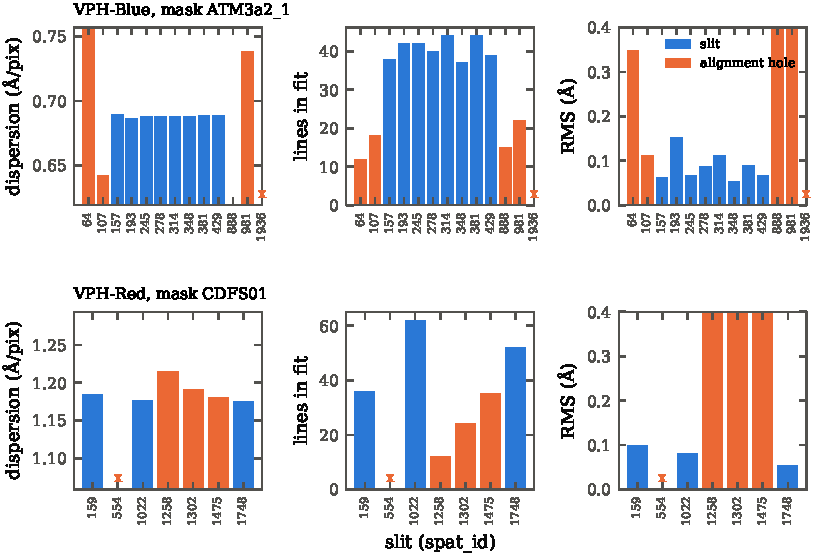
\includegraphics[width=\textwidth]{figures/mos_wavecal}
  \caption{Per-slit dispersion, number of lines used and fit RMS for the two
    multi-slit masks. Slits whose dispersion deviates by more than 5\,\% from the
    median are shown in orange.}
  \label{fig:mos_wavecal}
\end{figure}

\paragraph{Sky-line calibration.} For long VPH-Red exposures, the OH sky lines
provide an alternative calibration that is recorded through the same optical path
and at the same telescope position as the science data. We provide a sky-line
template for VPH-Red and a list of \nOHlines{} OH lines between 6000 and
\SI{10400}{\angstrom} (\code{OH\_LDSS3\_vac}; \cref{fig:sky}), derived from the
UVES sky atlas \citep{Hanuschik2003} and converted to vacuum. Unresolved
groups within \SI{3}{\angstrom} were merged to their flux-weighted centroid. The
parameters to enable this mode are given in \cref{app:quickstart}; the
flexure correction must then be disabled, since the solution is already in the
frame of the observation. This mode has not been validated end to end and is
not used in this report.

\begin{figure}[t]
  \centering
  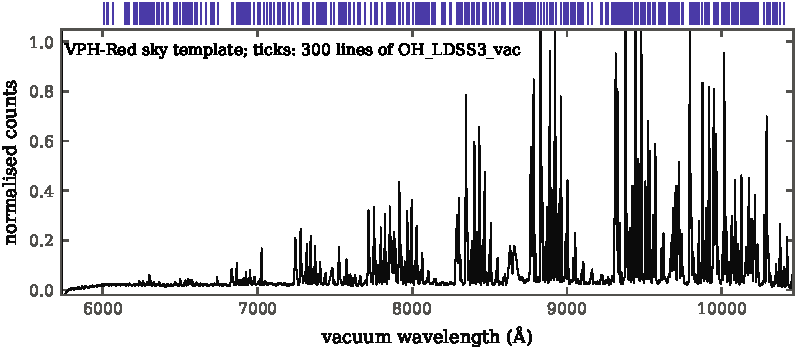
\includegraphics[width=\textwidth]{figures/sky_template}
  \caption{VPH-Red sky template with the positions of the \code{OH\_LDSS3\_vac}
    lines.}
  \label{fig:sky}
\end{figure}

%======================================================================
\section{Example reductions}
\label{sec:results}

\Cref{fig:science} shows, for each data set with science or standard-star
exposures, the sky-subtracted two-dimensional spectrum and the optimally extracted
one-dimensional spectrum of the object with the highest signal-to-noise ratio,
excluding alignment stars. The longslit standards reach $S/N>100$ per pixel. The
multi-slit targets are faint (knots of a lensed arc in ATM3a2\_1), with
$S/N\sim1$ per pixel in a single exposure, and are shown in 8-pixel bins.

The sky subtraction was assessed with the same $\chi$ statistic as in
\cref{sec:ron}, separately for the \SI{10}{\percent} of sky-dominated pixels with
the brightest sky and for the rest. In the longslit, $\sigma_\chi$ is
\chiFaintRedLS{} and \chiBrightRedLS{} respectively: sky subtraction is
noise-limited even on the brightest lines. In the multi-slit masks it is
\chiFaintBlueMOS{} and \chiBrightBlueMOS{} (ATM3a2\_1) and \chiFaintRedMOS{} and
\chiBrightRedMOS{} (CDFS01), and the distribution on bright lines has extended
tails: sky-line residuals exceed the noise by \SIrange{10}{20}{\percent}. These
residuals, visible as spikes at the OH lines in the faint spectra of
\cref{fig:science}, are typical of short slits (6--\SI{12}{arcsec}), where the
sky model has less spatial leverage, and should be considered when interpreting
features at bright sky lines.

\begin{figure}[p]
  \centering
  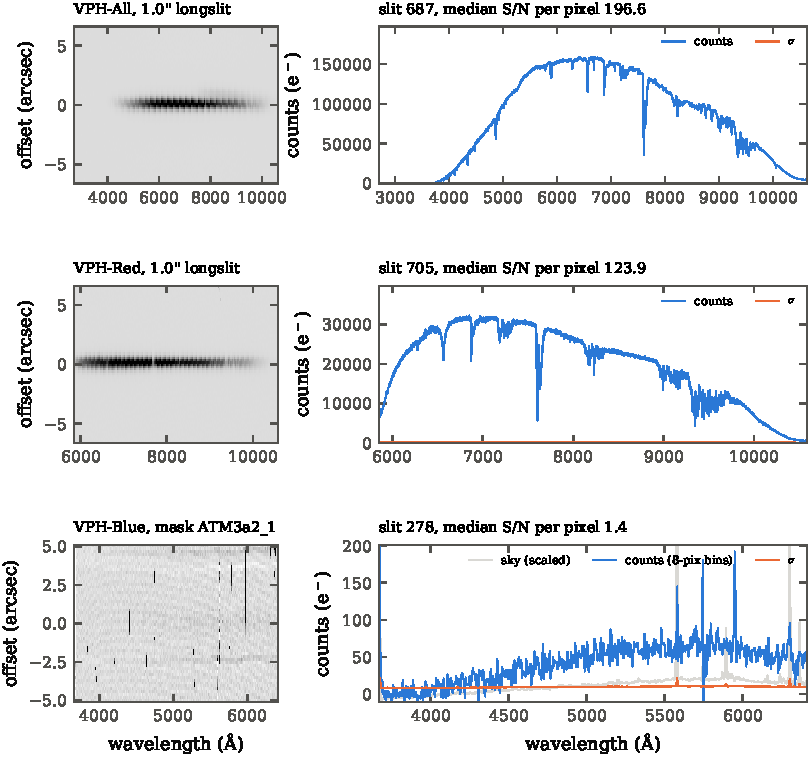
\includegraphics[width=\textwidth]{figures/science_examples}
  \caption{Examples of reduced data. Left: sky-subtracted two-dimensional
    spectrum around the object, with wavelength increasing to the right. Right:
    optimally extracted spectrum (blue) and its uncertainty (orange), in
    electrons, before flux calibration.}
  \label{fig:science}
\end{figure}

%======================================================================
\section{Recommendations for observers and for the observatory}
\label{sec:recommend}

\subsection*{For observers}
\begin{itemize}
  \item \textbf{Name frames consistently.} The \code{OBJECT} card drives the
    classification (\cref{tab:typing}). Include \code{arc}, \code{flat} (or
    \code{Qh}), \code{bias} or \code{dark} as a separate word in the names of
    calibration frames, e.g.\ ``arc CDFS01'', ``flat CDFS01''. Names such as
    ``NeHeAr'' are not recognised.
  \item \textbf{Take flats with the science filter.} Flats and arcs should be
    taken with the same grism, slitmask and order-blocking filter as the science
    frames. A change of filter defines a new configuration, and flats taken
    without the filter do not match the spectral shape of the science data.
  \item \textbf{Keep the two amplifier files together.} Both \code{c1} and
    \code{c2} files of every exposure are needed. If only one is available the
    pipeline reduces that half and reports it in the log.
  \item \textbf{Standards.} Standards and science frames are separated at
    \SI{100}{\second} by default; standards longer than this must be marked by
    hand or the limit changed.
  \item \textbf{Mask design.} Avoid placing slit edges on the bad columns of
    \cref{tab:bpm} (the region 1490--1700 of the trimmed frame is the most
    affected) and avoid slitlets shorter than \SI{\sim5}{arcsec}, whose arcs give
    unreliable wavelength solutions.
  \item \textbf{Alignment holes} are reduced as slits, with invalid wavelength
    solutions; ignore them (\cref{sec:holes}).
  \item \textbf{Flat exposure level.} Flats taken without the blocking filter
    saturate the alignment holes and are brighter than the science
    configuration requires; use the science filter and keep the slit
    illumination well below \SI{65000}{\adu}.
  \item \textbf{Check the output} with \code{ldss3\_qa.py}
    (\cref{app:quickstart}).
\end{itemize}

\subsection*{For the observatory}
\begin{itemize}
  \item \textbf{\code{ENOISE}.} The keyword reports 4.67 and 5.06~\si{\electron},
    close to the Slow-mode read noise, for Fast-mode data, underestimating the
    read noise by \ronExcessRange\,\%. It should reflect the readout mode.
  \item \textbf{\code{JD}.} The \code{JD} keyword cannot be used to derive the
    observation time; the pipeline computes the MJD from \code{UT-DATE} and
    \code{UT-TIME}.
  \item \textbf{\code{EXPTYPE}.} Arcs and flats are written with either
    \code{EXPTYPE = 'Flat'} or \code{'Object'}, and biases record the grism in
    the beam. A reliable exposure type (e.g.\ set from the lamp status) would
    make the classification independent of the observers' naming.
  \item \textbf{Documentation.} We suggest listing the bad-column ranges of
    \cref{tab:bpm} and the longslit bridge positions in the instrument manual.
\end{itemize}

%======================================================================
\section{Known limitations and future work}
\label{sec:issues}

\begin{itemize}
  \item Only $1\times1$ binning has been tested. Other binnings produce a
    warning; the data and overscan sections are then read from the header and
    should be checked.
  \item Alignment holes are traced and reduced as slits; they are flagged by
    \code{ldss3\_qa.py} but not excluded by the pipeline (\cref{sec:holes}).
    The mask design file could be used to identify them.
  \item Wavelengths are extrapolated beyond the reddest arc line of VPH-Red
    (\SI{\sim9790}{\angstrom}; validated with sky lines to \SI{0.4}{\angstrom}),
    blueward of the first line in slits whose coverage extends there, and
    blueward of \SI{3890}{\angstrom} with VPH-All, where there is no signal.
  \item VPH-All has been tested in longslit mode only. The VPH-Red multi-slit test
    used flats taken without the blocking filter.
  \item Sky-line residuals in short multi-slit slits exceed the noise by
    \SIrange{10}{20}{\percent} (\cref{sec:results}).
  \item Flux calibration has not been validated.
  \item The sky-line calibration mode has not been validated end to end.
  \item The implementation lives in a fork of \pypeit{}; we plan to contribute
    it to the main \pypeit{} repository, after which it will be installed with
    the standard \pypeit{} distribution.
\end{itemize}

%======================================================================
\appendix

\section{Default parameters}
\label{app:params}

\Cref{tab:params} lists the parameters that the LDSS3-C spectrograph class
changes from the \pypeit{} defaults. The complete parameter set of any
reduction is written to the \code{.par} file in the reduction directory.

\begin{longtable}{lll}
  \caption{Parameters set by the LDSS3-C spectrograph class that differ from the
    \pypeit{} defaults (\code{default\_pypeit\_par}). Grism-dependent settings
    (\code{config\_specific\_par}) are the wavelength template
    (\code{reid\_arxiv}), \code{method = full\_template}, \code{lamps = HeI, NeI,
    ArI}, and \code{fwhm} = 6 binned pixels; for longslit masks
    \code{sync\_predict = nearest}.}
  \label{tab:params}\\
  \toprule
  Parameter group & Parameter & Value \\
  \midrule
  \endfirsthead
  \toprule
  Parameter group & Parameter & Value \\
  \midrule
  \endhead
  \code{rdx} & \code{spectrograph} & \code{magellan\_ldss3} \\
  \code{darkframe} & \code{exprng} & \code{1, None} \\
  \code{arcframe} & \code{exprng} & \code{None, 60} \\
  \code{tiltframe} & \code{exprng} & \code{None, 60} \\
  \code{standardframe} & \code{exprng} & \code{None, 100} \\
  \code{flatfield} & \code{saturated\_slits} & \code{mask} \\
  \code{wavelengths} & \code{sigdetect} & \code{6.0} \\
  \code{wavelengths} & \code{fwhm} & \code{5.0} \\
  \code{wavelengths} & \code{rms\_thresh\_frac\_fwhm} & \code{0.5} \\
  \code{wavelengths} & \code{match\_toler} & \code{2.5} \\
  \code{wavelengths} & \code{n\_first} & \code{3} \\
  \code{wavelengths} & \code{n\_final} & \code{5} \\
  \code{slitedges} & \code{minimum\_slit\_length} & \code{2.0} \\
  \code{tilts} & \code{spat\_order} & \code{6} \\
  \code{tilts} & \code{spec\_order} & \code{6} \\
  \code{scienceframe} & \code{exprng} & \code{100, None} \\
  \code{scienceframe / process} & \code{sigclip} & \code{5.0} \\
  \code{scienceframe / process} & \code{objlim} & \code{2.0} \\
  \code{reduce / skysub} & \code{bspline\_spacing} & \code{0.8} \\
  \code{reduce / skysub} & \code{global\_sky\_std} & \code{False} \\
  \code{flexure} & \code{spec\_method} & \code{boxcar} \\
  \code{sensfunc} & \code{algorithm} & \code{IR} \\
  \code{sensfunc} & \code{polyorder} & \code{7} \\
  \code{sensfunc / IR} & \code{telgridfile} & \code{TellPCA\_3000\_26000\_R15000.fits} \\
  \bottomrule
\end{longtable}


\section{Header keywords}
\label{app:header}

\begin{table}[h]
  \centering\small
  \caption{Header keywords read by the pipeline.}
  \label{tab:header}
  \begin{tabular}{ll}
    \toprule
    Keyword & Use \\
    \midrule
    \code{OBJECT}, \code{EXPTYPE} & frame classification, target name \\
    \code{GRISM}, \code{APERTURE}, \code{FILTER}, \code{BINNING} & configuration \\
    \code{EXPTIME}, \code{AIRMASS}, \code{RA}, \code{DEC} & metadata \\
    \code{UT-DATE}, \code{UT-TIME} & observation time (MJD) \\
    \code{OPAMP}, \code{SPEED}, \code{EGAIN} & amplifier, readout mode, gain \\
    \code{DATASEC}, \code{BIASSEC} & data and overscan sections \\
    \bottomrule
  \end{tabular}
\end{table}

\section{Quick start}
\label{app:quickstart}

Install the fork in a fresh environment (Python~3.12):
\begin{lstlisting}
conda create -n ldss3 python=3.12 pip && conda activate ldss3
conda install -c conda-forge pyqt=6
git clone -b ldss3_multigrating https://github.com/joaquinhernandezg/PypeIt.git
cd PypeIt && pip install -e .
\end{lstlisting}
Inspect the raw data, write the input file for one configuration, check its
\code{frametype} column, and reduce:
\begin{lstlisting}
pypeit_setup -s magellan_ldss3 -r /path/to/raw
pypeit_setup -s magellan_ldss3 -r /path/to/raw -c A
cd magellan_ldss3_A && run_pypeit magellan_ldss3_A.pypeit
\end{lstlisting}
Useful additions to the parameter block of the \code{.pypeit} file:
\begin{lstlisting}
[reduce]
    [[findobj]]
        find_trim_edge = 100, 100   # multi-slit: ignore slit edges
[calibrations]
    [[standardframe]]
        exprng = None, 300          # standards up to 300 s
[scienceframe]
    exprng = 300, None
\end{lstlisting}
Sky-line wavelength calibration for VPH-Red (set the \code{frametype} of the
science frames to \code{arc,tilt,science}):
\begin{lstlisting}
[calibrations]
    [[wavelengths]]
        lamps = OH_LDSS3_vac
        method = full_template
        reid_arxiv = magellan_ldss3_vph_red_sky.fits
    [[arcframe]]
        exprng = 0, None
    [[tiltframe]]
        exprng = 0, None
[flexure]
    spec_method = skip
\end{lstlisting}
Quality assessment and visual inspection:
\begin{lstlisting}
python ldss3-qa/ldss3_qa.py magellan_ldss3_A --tar
pypeit_chk_wavecalib Calibrations/WaveCalib_*.fits
pypeit_chk_edges Calibrations/Edges_*.fits.gz
pypeit_show_2dspec Science/spec2d_*.fits
\end{lstlisting}

\section{Reproducing this report}
\label{app:repro}

The \code{report/} directory of \citet{ldss3_qa} contains the input files of
every reduction (\code{pypeit\_files/}) and the scripts that produce all
measurements, tables and figures:
\code{prepare\_pypeit\_files.py} and \code{run\_reductions.sh} (reductions),
\code{measure\_detector.py} (\cref{sec:detector}),
\code{measure\_calibs.py} (\cref{sec:procedure,sec:wavecal,sec:results}),
\code{make\_tables.py} and \code{make\_figures.py}. Running \code{make} in that
directory rebuilds the document. The reductions used \pypeit{} version
\code{\pypeitVersion}.

\bibliographystyle{plainnat}
\bibliography{refs}

\end{document}
